\subsection{Ablation study for GCF}
Meng Liu et. al does not present an ablation study for BiTGCF and GCF, which LightGCN showed is important with their regards to NGCF \cite{lightgcn,BiTGCF}.
In this section we conduct an ablation study on GCF to get an understanding on the effect of the different parts of the embedding propagation and layer combination.
Examples of the equations can be seen on \autoref{eq:GCF-minus-sc}, \autoref{eq:GCF-only-IP} and \autoref{eq:GCF-minus-IP}.
On \autoref{eq:GCF-minus-sc} the self-connection has been removed and is called \textit{GCF-minus-sc}.
On \autoref{eq:GCF-only-IP} only the inner product of the neighbor has been contained, and is called \textit{GCF-only-IP}
\autoref{eq:GCF-minus-IP} has the inner product been removed and is called \textit{GCF-minus-IP}.
There are also examples where GCF utilizes summation as layer combination as used in LightGCN which can be seen on \autoref{eq:lightgcn-sum}.
These are named \textit{GCF-sum}.
When LightGCN is tested with concatenation as layer combination it is called \textit{LightGCN-concat}
\begin{equation}
    \mathbf{e}_{u}^{(k+1)} = \sum^{}_{i \in \mathcal{N}_u}  \frac{1}{\sqrt{|\mathcal{N}_u||\mathcal{N}_i|}}\left( \mathbf{e}_i^{(k)} + \mathbf{e}_i^{(k)} \odot \mathbf{e}_u^{(k)} \right)
    \label{eq:GCF-minus-sc}
\end{equation}
\begin{equation}
    \mathbf{e}_{u}^{(k+1)} = \mathbf{e}_{u}^{(k)} + \sum^{}_{i \in \mathcal{N}_u}  \frac{1}{\sqrt{|\mathcal{N}_u||\mathcal{N}_i|}} \mathbf{e}_i^{(k)} \odot \mathbf{e}_u^{(k)}
    \label{eq:GCF-only-IP}
\end{equation}
\begin{equation}
    \mathbf{e}_{u}^{(k+1)} = \mathbf{e}_{u}^{(k)} + \sum^{}_{i \in \mathcal{N}_u}  \frac{1}{\sqrt{|\mathcal{N}_u||\mathcal{N}_i|}} \mathbf{e}_i^{(k)}
    \label{eq:GCF-minus-IP}
\end{equation}
\autoref{fig:GCF-NDCG-ablation-study} and \autoref{fig:GCF-recall-ablation-study} contains the GCF ablation study, where all GCF modifications still have the inner product between users and items, except for LightGCN.
The methods are as described here:\\
\begin{itemize}
    \item \textbf{GCF}: The original GCF method as described in \autoref{subsubsec:GCF-embed-propagation}.
    \item \textbf{GCF-minus-sc}: GCF without self connections
    \item \textbf{GCF-only-IP}:  GCF where $e_i^{(k)}$ has been removed in \autoref{eq:GCF-embedding}, so that GCF's graph convolutions only considers the inner product of users and items.
    \item \textbf{GCF-only-IP-minus-sc}: Implemented as GCF-only-ip but without self connections.
    \item \textbf{GCF-minus-IP}: GCF where inner product has been removed.
    \item \textbf{GCF-minus-IP-and-sc}: Same as GCF-minus-IP, but without self connections.
    \item \textbf{LightGCN-concat}: LightGCN with concatenation as layer combination.
    \item \textbf{LightGCN}: Original LightGCN as described in \autoref{subsubsec:LightGCN-embed-propagation}.
    \item \textbf{LightGCN-plus-sc}: LightGCN, but with self connections.
    \item \textbf{GCF-sum-only-IP}: Implemented as GCF-only-IP except that the layer combination method used is weighted summation.
    \item \textbf{GCF-sum}: GCF where the layer combination has been changed to weighted summation instead of concatenation.
    \item \textbf{GCF-sum-minus-sc}: Implemented as GCF-sum but without self connections.
\end{itemize}
\begin{figure}[h!]
    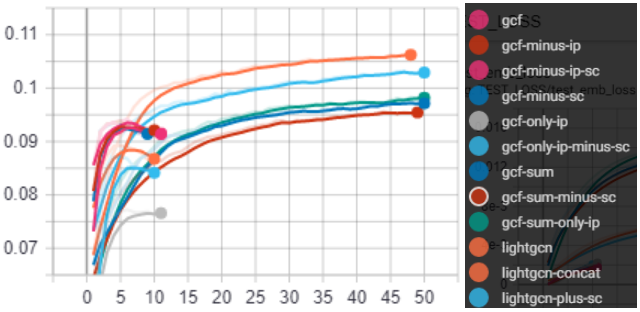
\includegraphics[width=\linewidth]{figures/gcf-all-ndcg.png}
    \caption{NDCG@50 for the Yelp2020 dataset.}
    \label{fig:GCF-NDCG-ablation-study}
\end{figure}
\begin{figure}[h!]
    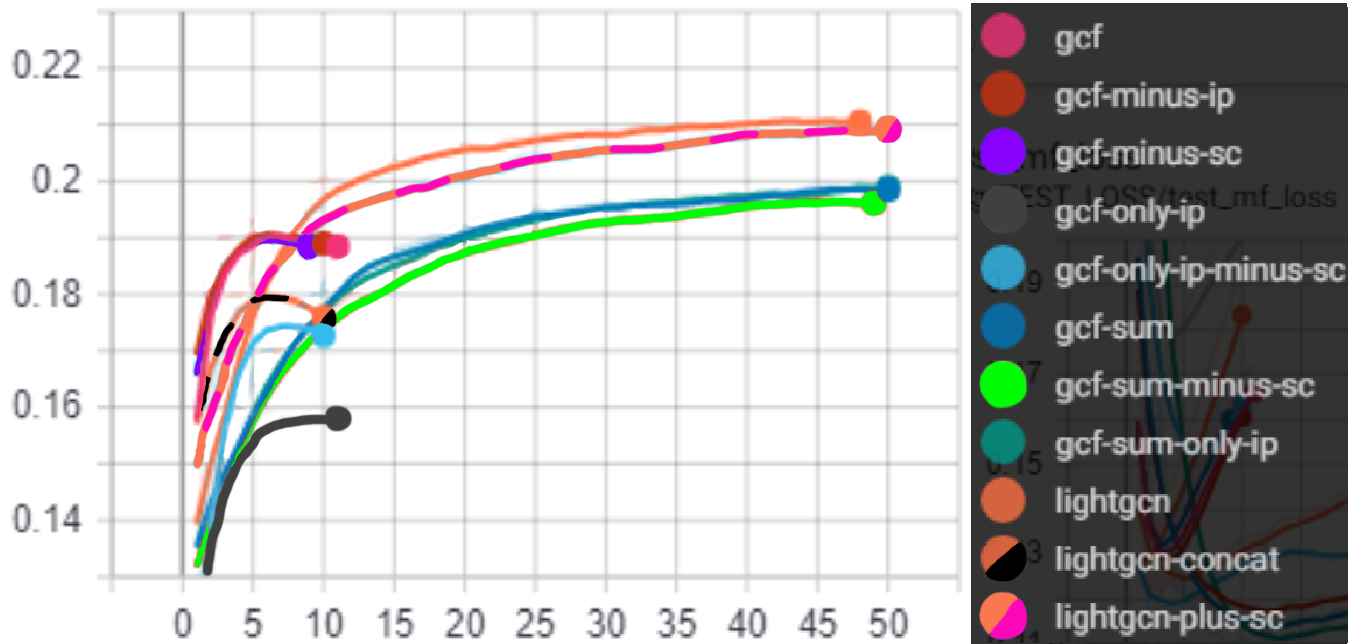
\includegraphics[width=\linewidth]{figures/gcf-all-recall.png}
    \caption{Recall@50 on the Yelp2020 dataset.}
    \label{fig:GCF-recall-ablation-study}
\end{figure}
From \autoref{fig:GCF-NDCG-ablation-study} and \autoref{fig:GCF-recall-ablation-study} it can be seen that the methods that do utilize concatenation as layer combination generally performs worse than the methods that utilize summation.
The results can also be seen on \autoref{tab:ablation-results}
It can also be seen that most concatenation methods learn faster than the summation methods.
For these experiments the dropout ratio is 0, so it could be because the concatenation methods hits overfitting.
Additionally we can see that convolutions of items and user are beneficial, when using concatenation as layer combination, but decreases performance when using weighted summation as layer combination, while combining it with inner product.
This is likely because weighted summation is more sensitive to changes in the embedding, and using both neighboring convolutions and inner product can create contradictions.
\begin{table}[]
    \centering
    \begin{tabular}{|l|l|l|}
        \hline
                             & NDCG    & Recall \\ \hline
        GCF                  & 0.09092 & 0.1869 \\ \hline
        GCF-minus-ip         & 0.09179 & 0.1881 \\ \hline
        GCF-minus-ip-sc      & 0.09087 & 0.1871 \\ \hline
        GCF-minus-sc         & 0.09084 & 0.1879 \\ \hline
        GCF-only-ip          & 0.07659 & 0.1587 \\ \hline
        GCF-only-ip-minus-sc & 0.08338 & 0.1712 \\ \hline
        LightGCN-concat      & 0.0856  & 0.1735 \\ \hline
        LightGCN             & 0.1064  & 0.2106 \\ \hline
        GCF-sum              & 0.09724 & 0.1988 \\ \hline
        GCF-sum-minus-sc     & 0.0956  & 0.1962 \\ \hline
        GCF-sum-only-ip      & 0.09843 & 0.199  \\ \hline
        LightGCN-plus-sc     & 0.1031  & 0.2098 \\ \hline
    \end{tabular}
    \caption{NDCG and Recall of the changed methods.}
    \label{tab:ablation-results}
\end{table}
\begin{figure}[h!]
    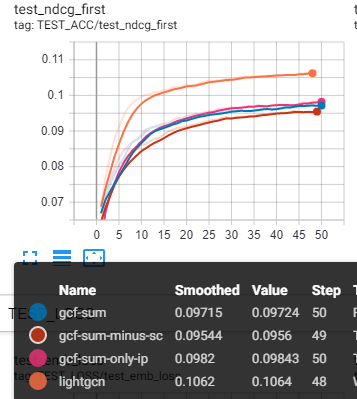
\includegraphics[width=\linewidth]{figures/gcf-sum-ndcg.png}
    \caption{NDCG@50 for the compared methods that utilize summation as layer combination on the Yelp2020 dataset.}
    \label{fig:GCF-sum-NDCG-ablation-study}
\end{figure}
\begin{figure}[h!]
    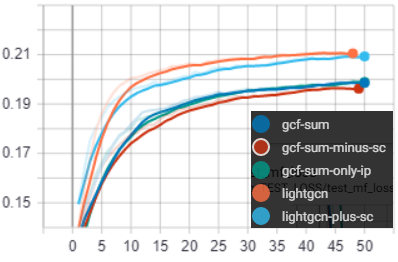
\includegraphics[width=\linewidth]{figures/gcf-sum-recall.png}
    \caption{Recall@50 on the compared methods that utilize summation as layer combination on the Yelp2020 dataset.}
    \label{fig:GCF-sum-recall-ablation-study}
\end{figure}
Looking at \autoref{fig:GCF-sum-NDCG-ablation-study} and \autoref{fig:GCF-sum-recall-ablation-study} it can be seen that LightGCN performs better than the other GCF methods that utilize weighted summation as layer combination.
\begin{figure}[h!]
    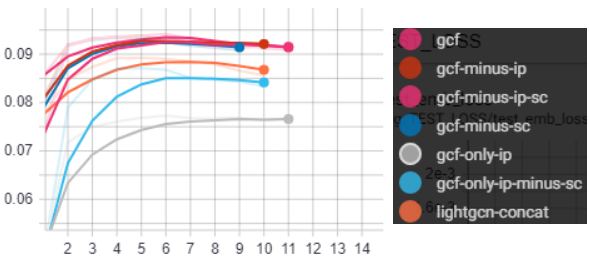
\includegraphics[width=\linewidth]{figures/gcf-ndcg-concat.png}
    \caption{NDCG@50 for the compared methods that utilize concatenation as layer combination on the Yelp2020 dataset.}
    \label{fig:GCF-NDCG-concat-ablation-study}
\end{figure}
\begin{figure}[h!]
    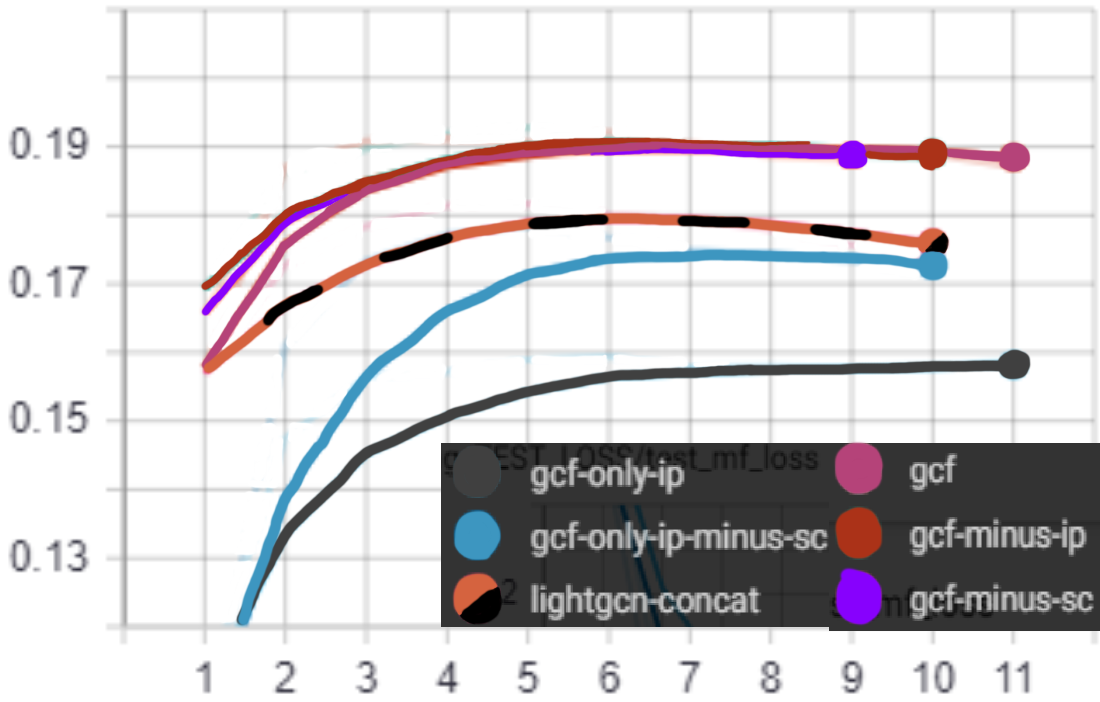
\includegraphics[width=\linewidth]{figures/gcf-concat-recall.png}
    \caption{Recall@50 for the compared methods that utilize concatenation as layer combination on the Yelp2020 dataset.}
    \label{fig:GCF-recall-concat-ablation-study}
\end{figure}
On \autoref{fig:GCF-NDCG-concat-ablation-study} and \autoref{fig:GCF-recall-concat-ablation-study} GCF without self connections performs a small amount better than GCF.
Removing inner product or only keeping inner product makes them perform worse when using concatenation as layer combination.
Interestingly \textit{gcf-only-ip-minus-sc} performs better than \textit{gcf-only-ip}, which can indicate that self connections are harmful for performance, if you only use inner product in the convolutions.
